% Created 2025-10-09 Thu 06:54
% Intended LaTeX compiler: xelatex
\documentclass[professionalfonts,11pt]{beamer}
\usepackage{graphicx}
\usepackage{longtable}
\usepackage{wrapfig}
\usepackage{rotating}
\usepackage[normalem]{ulem}
\usepackage{capt-of}
\usepackage{hyperref}
\usepackage{color}
\usepackage{minted}
\setlength{\paperwidth}{17in}
\setlength{\textwidth}{15in}
\setlength{\paperheight}{11in}
\setlength{\textwidth}{9in}
\usepackage{amssymb}
\usetheme{metropolis}
\usecolortheme{default}
\metroset{
block=fill,
numbering=fraction,
progressbar=foot,
titleformat=smallcaps,
sectionpage=progressbar
}
\usepackage{fontspec}
\setmonofont{DejaVu Sans Mono}
\usepackage{setspace}
\onehalfspacing
\usepackage{booktabs}
\usepackage[table]{xcolor}
\usepackage{colortbl}
\usepackage{sectsty}
\usepackage{soul}
\usepackage{microtype}
\usepackage{siunitx}
\usepackage{physics}
\usepackage[tikz]{bclogo}
\setcounter{MaxMatrixCols}{20}
\usepackage{minted,xcolor}
\usemintedstyle{manni}
\definecolor{bg}{HTML}{ffffe6}
\setminted{bgcolor=bg,linenos}
\definecolor{TyrianPurple}{HTML}{66023C}
\definecolor{Tiffany}{HTML}{00FFDD}
\setbeamercolor{alerted text}{fg=TyriannPurple}
\setbeamercolor{frametitle}{bg=TyrianPurple,fg=white}
\setbeamercolor{section in toc}{fg=TyrianPurple}
\setbeamercolor{progress bar in head/foot}{fg=TyrianPurple,bg=gray!30}
\setbeamerfont{frametitle}{series=\bfseries,size=\large}
\setbeamertemplate{frametitle}{
\vspace*{0.5em}
\nointerlineskip
\begin{beamercolorbox}[wd=\paperwidth,ht=2.5ex,dp=1.0ex,leftskip=1em]{frametitle}
\usebeamerfont{frametitle}\insertframetitle
\end{beamercolorbox}
}
\usepackage{tikz}
\usetheme{default}
\author{Michael Raba, MSc Candidate University of Kentucky '25}
\date{\today}
\title{Michael Raba Portfolio Fall 25}
\hypersetup{
 pdfauthor={Michael Raba, MSc Candidate University of Kentucky '25},
 pdftitle={Michael Raba Portfolio Fall 25},
 pdfkeywords={},
 pdfsubject={},
 pdfcreator={Emacs 29.1 (Org mode 9.7.34)}, 
 pdflang={English}}
\usepackage{biblatex}

\begin{document}

\maketitle
\begin{frame}[label={sec:orgad061ea}]{Multichamber Muffler}
\begin{columns}
\begin{column}{0.88\columnwidth}
\textbf{Insertion Loss for Multichamber vs Competing Mufflers}
\begin{itemize}
\item Goal: maximize Insertion Loss
\begin{itemize}
\item Insertion loss is the reduction in signal power (e.g., sound or RF) caused by inserting a device into a system, whereas transmission loss measures the total reduction in signal as it passes through a medium or barrier, independent of any added device.
\item IL isolates the muffler’s effect, letting evaluate designs without being affected by other parts of the exhaust/environment
\end{itemize}
\end{itemize}

\begin{figure}[htbp]
\centering
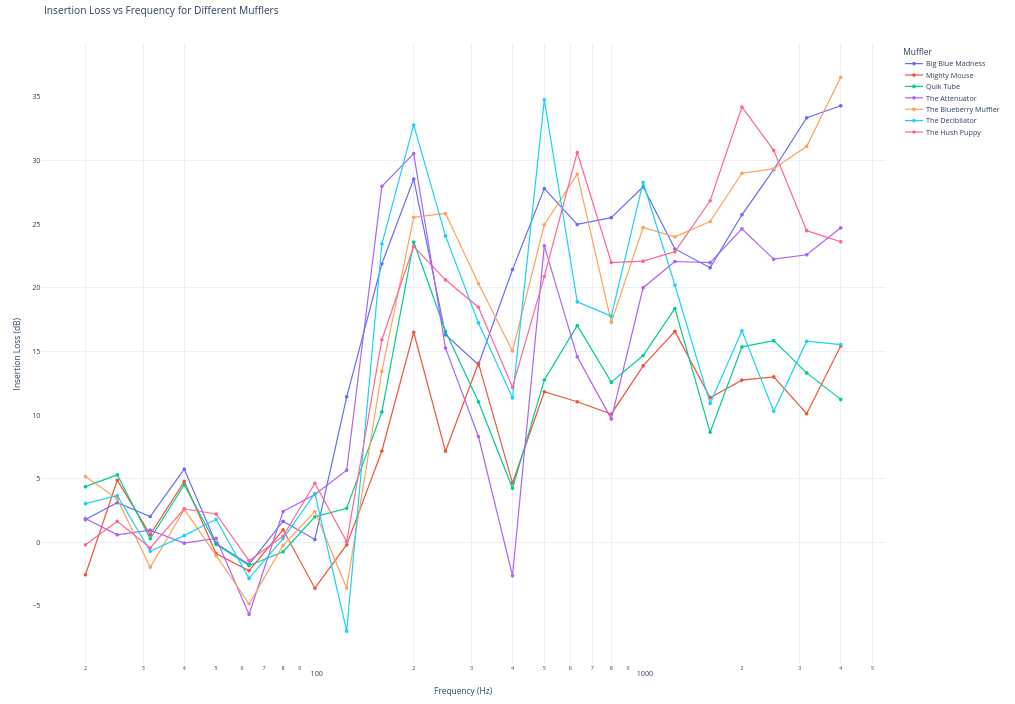
\includegraphics[width=0.7\textwidth]{./muff.il.png}
\caption{Insertion Loss for Muffler Competition}
\end{figure}

\begin{figure}[htbp]
\centering
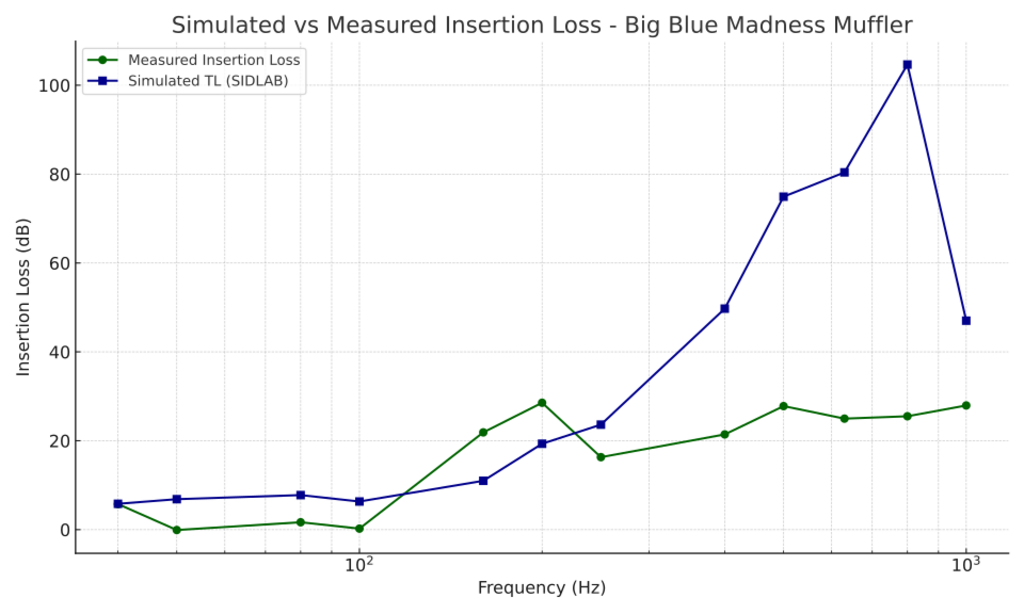
\includegraphics[width=0.7\textwidth]{../510finalProj/imag/bbm.png}
\caption{Sidlab 1d Insertion Loss Approximation (Transfer Matrix system)}
\end{figure}



\begin{align}
\text{IL}_\text{Big Blue Madness}(f) &= L_\text{straight}(f) - L_\text{Big Blue Madness}(f)
\end{align}     
\end{column}
\begin{column}{0.88\columnwidth}
\begin{figure}[htbp]
\centering
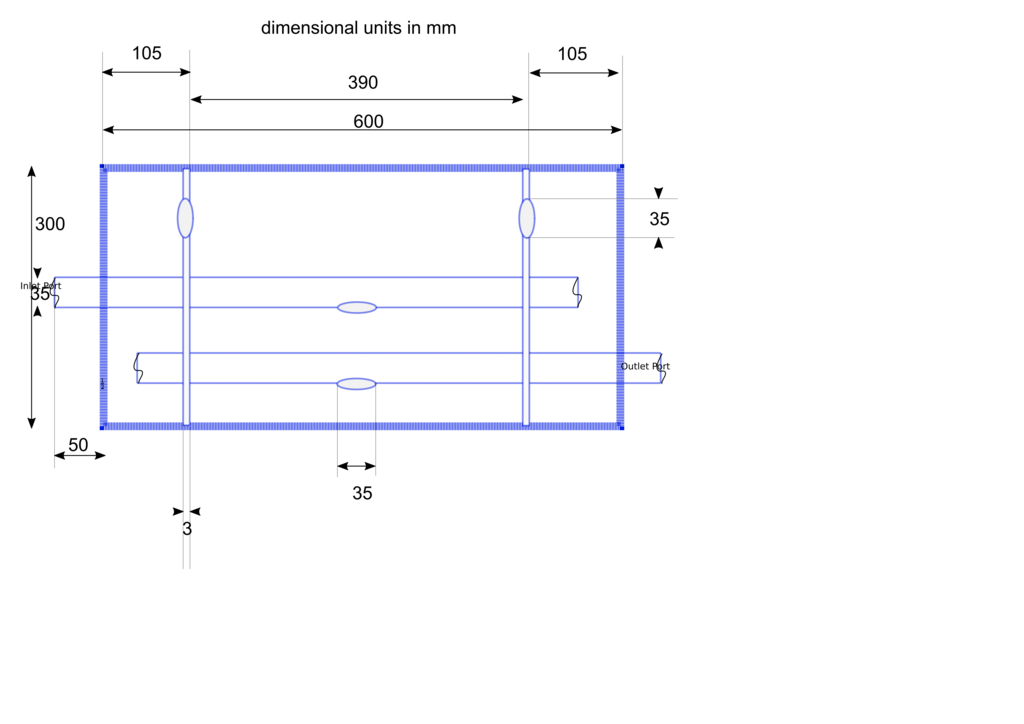
\includegraphics[width=0.5\textwidth]{./schematicMuf.png}
\caption{Schematic}
\end{figure}

\begin{figure}[htbp]
\centering

\includegraphics[width=0.6\textwidth]{./images/screenshot-02.png}
\caption{Multicomponent Muffler Internal Geometry (Ansys Workbench/Acoustics Module)}
\end{figure}


\begin{figure}[htbp]
\centering
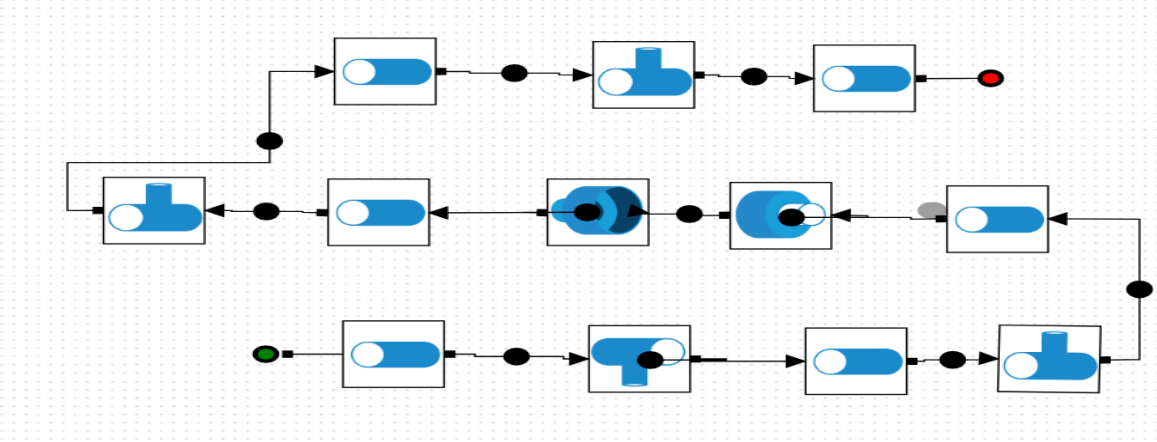
\includegraphics[width=0.7\textwidth]{../510finalProj/imag/sid1.png}
\caption{Sidlab 1d approximation (Transfer Matrix system)}
\end{figure}
\end{column}
\end{columns}
\end{frame}
\begin{frame}[label={sec:orge663848}]{Anand Model: Viscoelastoplasticity and its Application to Solder Joints}
\begin{columns}
\begin{column}{0.88\columnwidth}
\begin{figure}[htbp]
\centering
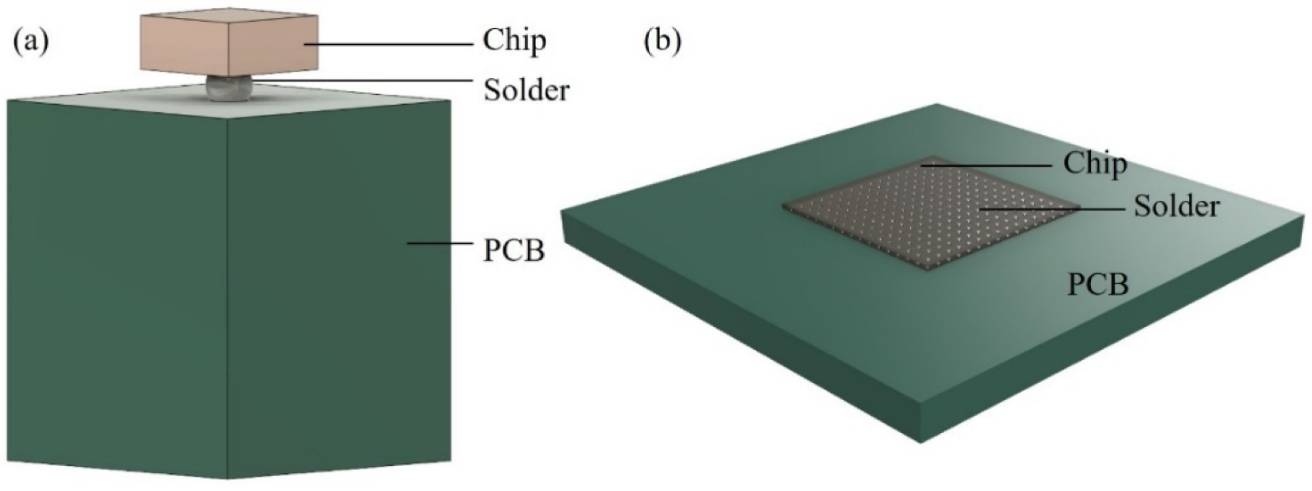
\includegraphics[width=.9\linewidth]{../603talk/chip.png}
\caption{Anand Viscoplasticity model applied to electronics packaging (pcb).}
\end{figure}
\begin{block}{Models Viscoplastic (Metals under Temperature/thermal cycling)}
\begin{itemize}
\item \textbf{Broad Application:} \alert{Model metals under thermal cycling! Temperature and Strain dependance!}
\item Applies Anand’s unified viscoplastic framework to model solder behavior
\item Anand's model can be reduced and fitted from experiments
\item transition the theory into engineering-scale implementation
\item Targets solder joints in microelectronic packages (chip on PCB, soldered connections)
\end{itemize}
\end{block}
\begin{block}{Viscoplastic System of Equations (Anand)}
\begin{align}
\text{Flow Rule (Plastic Strain Rate):} \quad
\dot{\varepsilon}^p &= A \exp\left( -\frac{Q}{R T} \right)
\left[ \sinh\left( \frac{j \, \sigma}{s} \right) \right]^{1/m}, \\
&\text{Plastic strain rate increases with stress and temperature,} \notag \\
&\text{No explicit yield surface; flow occurs at all nonzero stresses.} \notag
\end{align}



\begin{align}
\text{Deformation Resistance Saturation } s^*: \quad
s^* &= \hat{s} \left( \frac{\dot{\varepsilon}^p}{A} \exp\left( \frac{Q}{R T} \right) \right)^n, \\
&\text{Defines the steady-state value that } s \text{ evolves toward,} \notag \\
&\text{Depends on strain rate and temperature.} \notag
\end{align}

\begin{align}
\text{Evolution of Deformation Resistance } s: \quad
\dot{s} &= h_0 \left| 1 - \frac{s}{s^*} \right|^a
\, \text{sign}\left(1 - \frac{s}{s^*}\right) \dot{\varepsilon}^p, \\
&\text{Describes dynamic hardening and softening of the material,} \notag \\
& s \text{ evolves depending on proximity to } s^* \text{ and flow activity.} \notag
\end{align}

\noindent
\textit\{Note: Constants \(A, Q, m, j, h_0, \hat{s}, n, a\) are material-specific and fitted to experimental creep/strain rate data.\}
\end{block}
\end{column}
\begin{column}{0.88\columnwidth}
\begin{figure}[htbp]
\centering
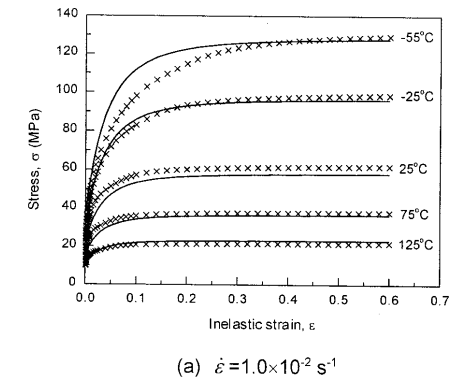
\includegraphics[width=0.5\textwidth]{../603talk/wMPa.png}
\caption{strain-rate and temperature dependence of solder materials (Source: Wang 2001 Paper)}
\end{figure}

\begin{figure}[htbp]
\centering
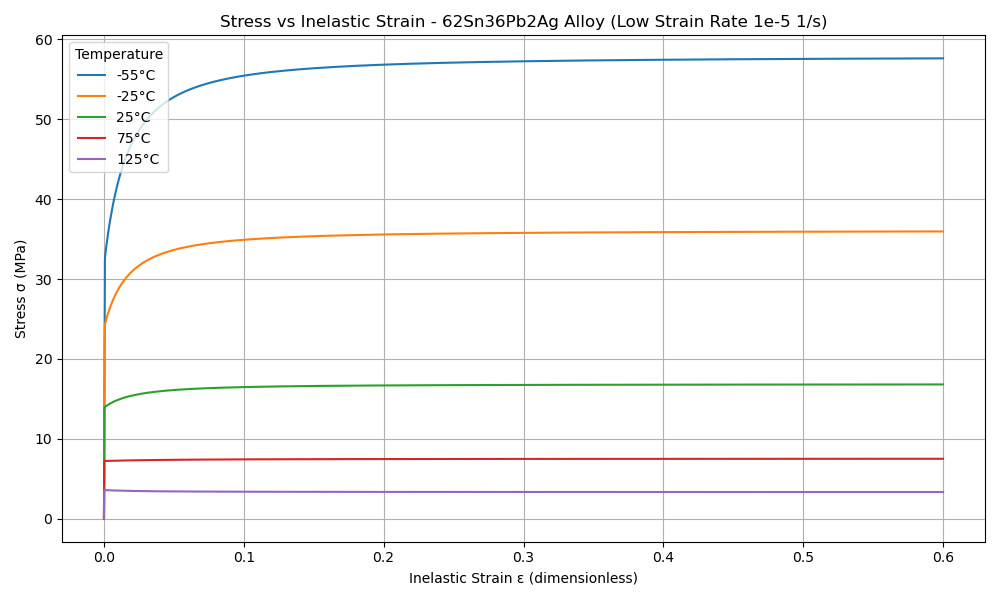
\includegraphics[width=0.7\textwidth]{../603talk/stress_vs_strain_62Sn36Pb2Ag.png}
\caption{Running model using Forward Euler code}
\end{figure}
\end{column}
\end{columns}
\end{frame}
\begin{frame}[label={sec:orgf74ef22}]{Turbulence Suppression (SVD-FFT Method)}
\begin{columns}
\begin{column}{0.88\columnwidth}
\begin{figure}[htbp]
\centering

\includegraphics[width=0.5\textwidth]{../MScUpdated/images/baileyedit/screenshot2023-04-15_10-45-50_.png}
\caption{Decompose turbulent pipe flow (Reynolds number \(Re=5300\) and \(Re=11,700\)) to Modal FFT/POD decomposition}
\end{figure}

\begin{center}

\includegraphics[width=0.5\textwidth]{../MScUpdated/images/baileyedit/screenshot2023-04-15_10-47-35_.png}
\end{center}

\begin{itemize}
\item Idea: Reduce turbulent flow to FFt-POD so it can be easily studied. The lowest POD modes have the most energy \(\therefore\) most important
\item Relaminarization occurs by suppression of near-wall vortices and streak breakdown.
\item Applications: rotating heat exchangers, turbomachinery, compact fluid systems.
\end{itemize}
\end{column}
\begin{column}{0.88\columnwidth}
\begin{figure}[htbp]
\centering

\includegraphics[width=0.5\textwidth]{./images/screenshot-03.png}
\caption{Fluid field in streamwise direction \(\textbf{u}_w\)}
\end{figure}



\begin{figure}[htbp]
\centering
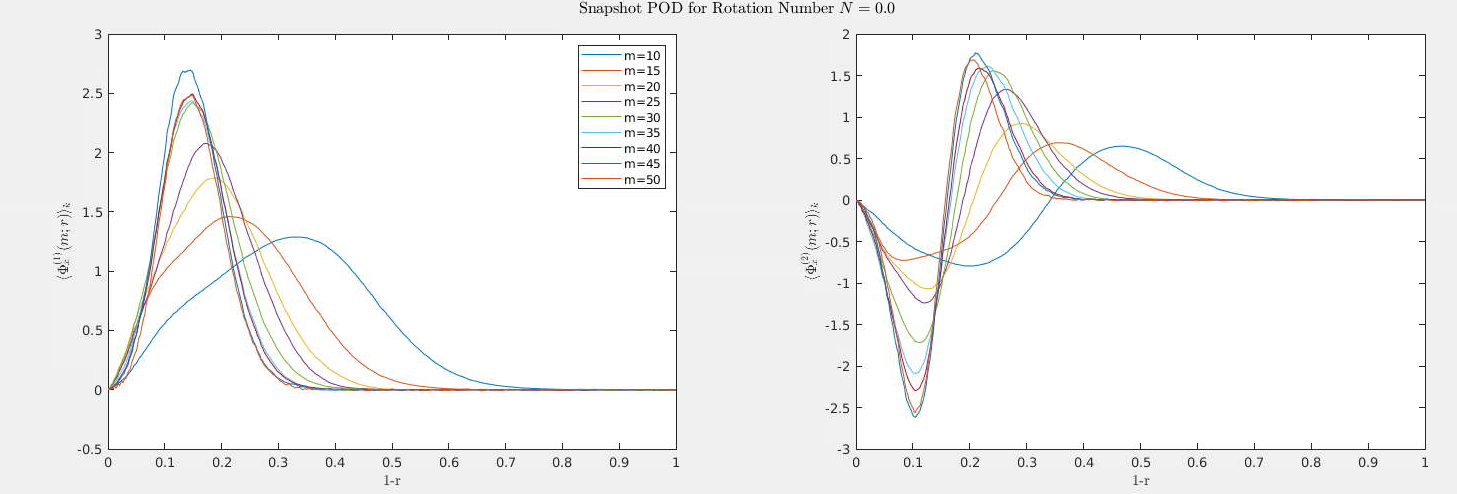
\includegraphics[width=0.7\textwidth]{../origPODtalks/images/reveal/screenshot2023-01-05_13-26-09_.png}
\caption{Turbulent Flow}
\end{figure}

\begin{figure}[htbp]
\centering
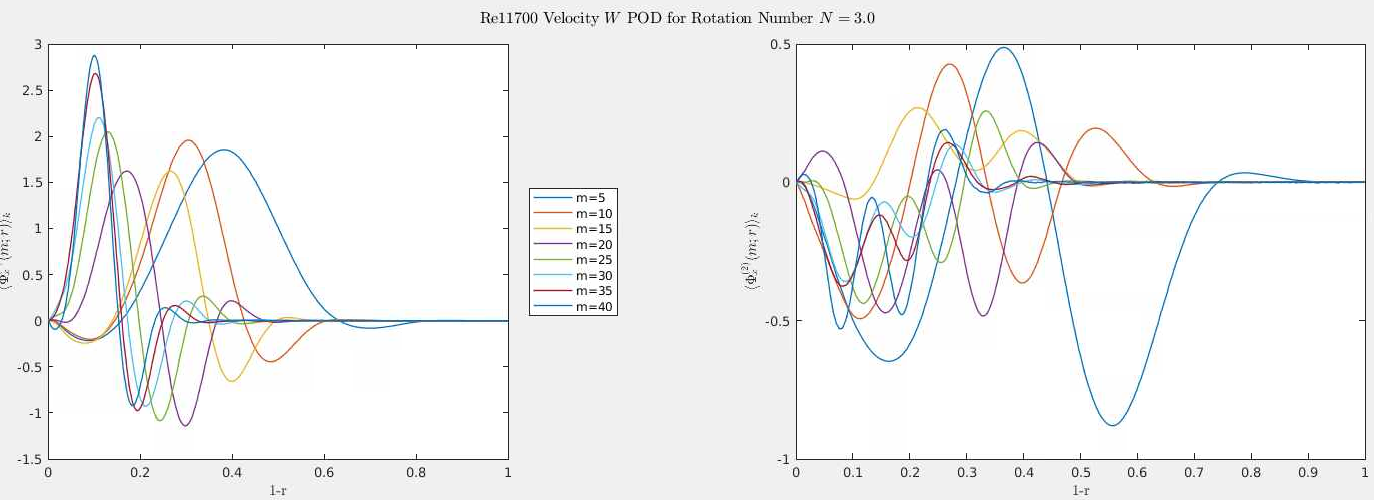
\includegraphics[width=0.7\textwidth]{../origPODtalks/images/baileyedit/screenshot2023-04-15_10-48-49_.png}
\caption{Relaminarized flow (Broadband Energy Distribution)}
\end{figure}
\end{column}
\end{columns}
\end{frame}
\begin{frame}[label={sec:org6ceecef}]{Selected Relevent Coursework (ME 514 Machine Design using Ansys Workbench, Fall 2024)}
\begin{columns}
\begin{column}{0.88\columnwidth}
\begin{block}{Microgripper Design}
\begin{itemize}
\item ME 514: A microgripper is a small-scale mechanical device designed to grasp, manipulate, or position micro-sized objects, often used in biomedical, microassembly, and MEMS applications.
\item Our design goal is to optimize the flexible gripper geometry to maximize Geometric Advantage (GA) while maintaining structural reliability (stress ≤ 15 MPa).
\item \alert{Geometric Advantage (GA)} is a performance metric defined as the ratio of the output displacement to the input displacement, indicating how effectively the gripper amplifies motion.
\end{itemize}
\end{block}
\begin{block}{Set Objective \& Constraints}
\begin{itemize}
\item Objective: Maximize deformation (improve GA).
\item Constraint: Stress ≤ 15 MPa.
\item Optimization Method: Adaptive Single-Objective (gradient-based) to \alert{Maximize GA (via X-axis deformation)}
\end{itemize}
\end{block}
\begin{block}{Output Parameters}
\begin{center}
\begin{tabular}{ll}
Parameter & Description\\
\hline
X-axis Directional Deformation & Objective (linked to GA)\\
Minimum Combined Stress & Constraint check\\
Maximum Combined Stress & Constraint check\\
\end{tabular}
\end{center}


\begin{figure}[h]
\centering
\begin{minipage}{0.45\textwidth}
  \centering
  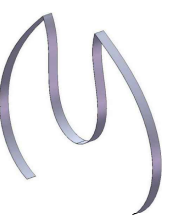
\includegraphics[width=0.9\textwidth]{./images/screenshot-05.png}
  \caption{Microgripper shape}
\end{minipage}\hfill
\begin{minipage}{0.45\textwidth}
  \centering
  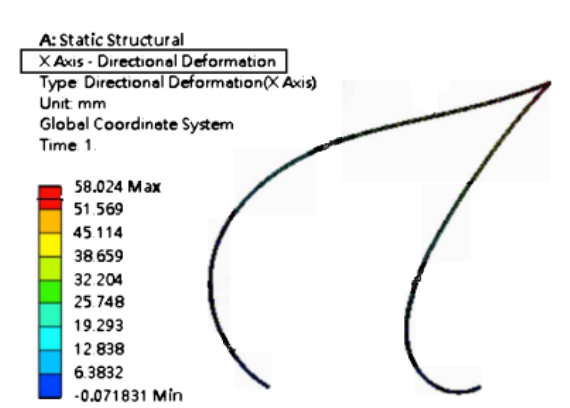
\includegraphics[width=0.9\textwidth]{./images/screenshot-07.png}
  \caption{Input parameters for optimization}
\end{minipage}
\end{figure}
\end{block}
\end{column}
\begin{column}{0.88\columnwidth}
Thread and Bolt Design with Ansys

\begin{itemize}
\item Assume coefficeint of friction between bolt  and nut \(=0.2\), mirror symmetry, and 2d simulation to reduce computation
\end{itemize}

\begin{figure}[htbp]
\centering
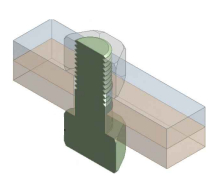
\includegraphics[width=0.3\textwidth]{./images/screenshot-08.png}
\caption{Threaded nut and bolt}
\end{figure}

\begin{figure}[htbp]
\centering
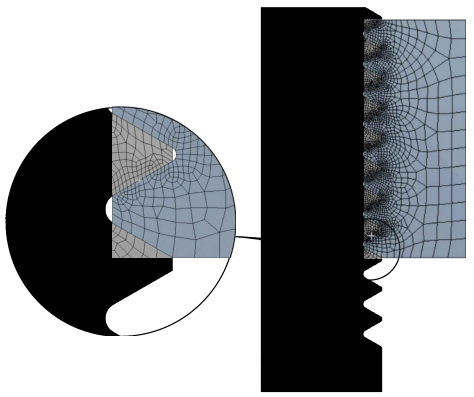
\includegraphics[width=0.3\textwidth]{./images/screenshot-10.png}
\caption{Mesh}
\end{figure}
\end{column}
\end{columns}
\end{frame}
\begin{frame}[label={sec:org90f3a8d}]{Selected Relevent Coursework (ME 514 Machine Design using Ansys Workbench, Fall 2024)}
\begin{columns}
\begin{column}{0.88\columnwidth}
\begin{figure}[htbp]
\centering
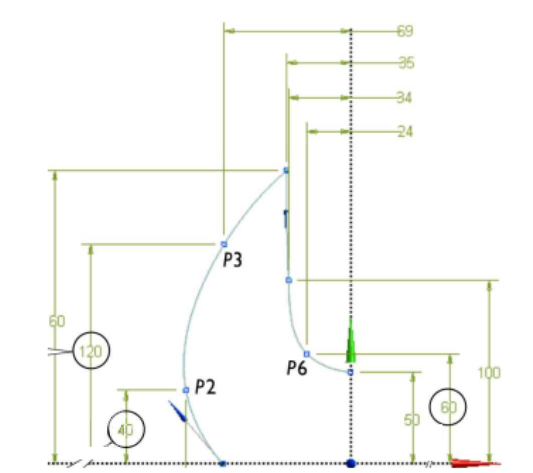
\includegraphics[width=0.6\textwidth]{./images/screenshot-04.png}
\caption{Design points \(P3, P2,P6\).}
\end{figure}
\begin{block}{Gripper (continued)}
Goal is to optimize geometry so it could amplify motion efficiently (maximize Geometric Advantage) while keeping stresses within safe limits.
\begin{itemize}
\item input motion at the actuator is small, amplifying motion achieves the displacement

\begin{itemize}
\item If \(GA>1\)
\end{itemize}
\item \alert{P2:} Controls the curvature near the base of the gripper arm.
\begin{itemize}
\item influences stiffness and how the arm starts to bend under load
\end{itemize}
\item \alert{P3:} located mid-span of gripper arm
\begin{itemize}
\item largest range of motion, affects overall flexibility and amplification
\item near tip and fine tunes end geometry, impacts contact alignment and stress distribution at the gripping point
\end{itemize}
\end{itemize}
\end{block}
\end{column}
\begin{column}{0.88\columnwidth}
Thread and Bolt Design with Ansys

Improving efficiency involves redistributing some of the load to upper threads to reduce maximum stress and enhance overall performance
\begin{center}
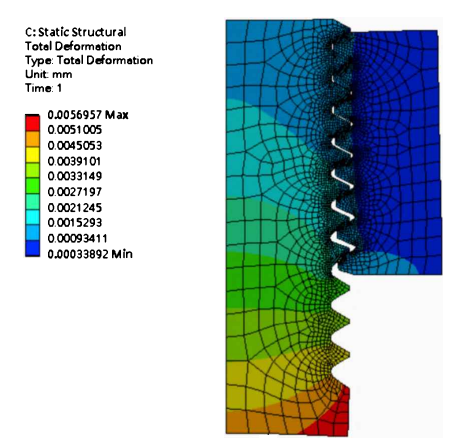
\includegraphics[width=0.8\textwidth]{./images/screenshot-11.png}
\caption{\textbf{uneven stress distribution} most stress concentrated on a few lower threads.}
\end{center}
\end{column}
\end{columns}
\end{frame}
\end{document}
